\documentclass[10pt, letterpaper]{article}

% Language setting
% Replace `english' with e.g. `spanish' to change the document language
\usepackage[english]{babel}

% Set page size and margins
% Replace `letterpaper' with`a4paper' for UK/EU standard size
\usepackage[letterpaper,top=2cm,bottom=2cm,left=3cm,right=3cm,marginparwidth=1.75cm]{geometry}

% Useful packages



\usepackage{fancyvrb}
\usepackage{fancyhdr, lastpage}
\pagestyle{fancy}
\lhead{Parker Levesque}
\rhead{CTA200H}
\cfoot{Page \thepage\ of \pageref{LastPage}}

\usepackage[Glenn]{fncychap}
%Options: Sonny, Lenny, Glenn, Conny, Rejne,
%Bjarne, Bjornstrup

\usepackage{xcolor}

\usepackage{tikz, tcolorbox}

\usepackage{physics}
\usepackage{amsmath,amsthm,amssymb}
\usepackage[dvips,letterpaper,margin=1.1in,bottom=0.7in]{geometry}
\usepackage{graphicx}
\usepackage{hyperref}
\hypersetup{
    colorlinks=true,
    linkcolor=blue,
    urlcolor=red,
    pdftitle={Template}
    }
\usepackage{enumitem}
\usepackage{charter}
\usepackage{tabstackengine}
\usepackage{siunitx}
\usepackage[font=small,labelfont=bf]{caption}
\usepackage{mwe}
\usepackage[sorting=none]{biblatex}



\usepackage{caption}

\usepackage{listings}
\usepackage{subcaption}
\usepackage{wrapfig}
\usepackage{indentfirst}
\usepackage{float}
\usepackage{geometry}
\usepackage{lipsum}
\usepackage[nice]{nicefrac}
\counterwithin{figure}{section}

\DeclareCaptionFont{white}{\color{white}}
\DeclareCaptionFormat{listing}{%
  \parbox{\textwidth}{\colorbox{gray}{\parbox{\textwidth}{#1#2#3}}\vskip-4pt}}
\captionsetup[lstlisting]{format=listing,labelfont=white,textfont=white}
\lstset{frame=lrb,xleftmargin=\fboxsep,xrightmargin=-\fboxsep}


\newcommand{\ds}{\displaystyle}

\title{Project - Interest Trends in Astrophysics}
\author{Parker Levesque \\ parker.levesque@mail.utoronto.ca}

\date{May, 2022}

\begin{document}



\maketitle
\vspace{1cm}

\section{Summary}

The goal of this project is to investigate the growth of interest in low surface brightness galaxies. This will be done using metrics from the astrophysics data system (ads), retrieved using the ads python package.

The first part of this project will be to characterize `interest'. There are three main metrics that can be used in order to assign a certain level of interest when it comes to topics or subject matter in the field of astronomy: number of citations, number of papers published, and number of reads. It is difficult to narrow down interest levels and compare them between two topics, however, it is straight foreword to say that the more people are citing, reading and publishing papers related to a topic, the more the scientific community is interested as a whole.


To continue, we will reduce this data in order to discover, analyse and compare trends. For relatively new topics in astronomy, such as low surface brightness galaxies (LSBG), it can be predicted that the interest will be low and spike in the recent years. All the while more dated topics may show interesting dynamics influenced by later discoveries, causing a resurgence in interest. 

\section{Using the ADS Package}

\textbf{Getting an API key and installing the package}: Creating an account with the \href{https://ui.adsabs.harvard.edu}{ADS} will provide a personal API key needed to use the python package. Saving the key to \color{blue} $\sim$/.ads/dev\_key \color{black} and running \color{blue} pip install ads \color{black} in the command line will set everything up. \\[5mm]

\textbf{Searching the Database}: The important function used to search the ADS database is the \textbf{SearchQuery()} function from the ads package. Many arguments can be used to specify a query, telling the function to gather a list of papers that have been registered containing these parameters. The relevant arguments for this project are:
\begin{itemize}
    \item \textbf{q}  -  Query the registered papers using keywords in substructures of the text. (e.g. title, abstract, body, year.)
    \item \textbf{sort} - Sorting the returned list of identified papers using a specified metric (e.g. citation count or read count)
    \item \textbf{fl} - Limiting the attributes fetched by the query. This helps control the rate limit usage when creating a request to the API. (e.g. title, abstract, body, citation count, read count) 
\end{itemize}

\vspace{2cm}

Information about the papers can then be used in python through the attributes. A simple example to demonstrate a title search: \\[5mm]

\begin{lstlisting}[language=python, label= Simple Example]
import ads

papers_2020 = ads.SearchQuery(q='title: galaxy year: 2020',
                sort='read_count', fl=['title', 'read_count']

for paper in papers_2020:
    print(paper.title, paper.read_count)
\end{lstlisting}

\vspace{0.5cm}

\section{The ads\_query\_pkg Package}

This package, created for this project, contains four functions designed to illustrate the overall interest in a certain topic, as well as the evolution of the interest over a specified period of time.

\subsection{cite\_count() and read\_count()}

The \textbf{cite\_count} function will arrange the all-time most cited papers, given a keyword, from most to least cited. It returns the citation counts arranged in that same order. The keyword can be specified to search in the title of the paper, the abstract, or both. The \textbf{read\_count()} function will do the same but using the read count of the papers instead.

This property will show an overall representation of the interest of a given topic; getting an idea of how many greatly influential papers that have been published, and the degree to which they have influenced the scientific community.

\subsection{top\_cite() and num\_papers()}

These two functions take a keyword input and a time frame (in years). The time frame is divided into a number of time periods (decades by default), and the functions will return the total number of citations or reads in each of the time periods respectively. Again, the keyword can be specified to search in the title of the paper, the abstract, or both.

This information will show when the general interest in the topic was sparked and how it has evolved over the desired time frame. This is especially useful when comparing two underlying subjects within the umbrella of a general topic. (e.g. black-holes vs worm-holes, under the topic of general relativity.).


\section{Analysing Trends and Comparing Interest}

For this analysis, we will be comparing growth in interest in different subject areas related to low surface brightness galaxies.

\vspace{1cm}
\textbf{Case Study: Dark Matter and Ultra-Diffuse Galaxies}
\vspace{1cm}

Due to the observed rotation curves and mass-to-light ratios of LSBGs, we know that they are dark matter dominated, making them great objects to further investigate the properties of dark matter. 

The term `Ultra-Diffuse galaxy', coined by Dr Abraham, is a galaxy that is on the extreme end of the low-surface-brightness spectrum. Some are known to contain mostly dark matter, while others are known to contain no dark matter at all.

Let's analyse the growth in interest related to these two subject areas, which are both connected to LSBGs in their own ways.

\begin{figure}[H]
    \hspace*{-5mm}
        \centering
        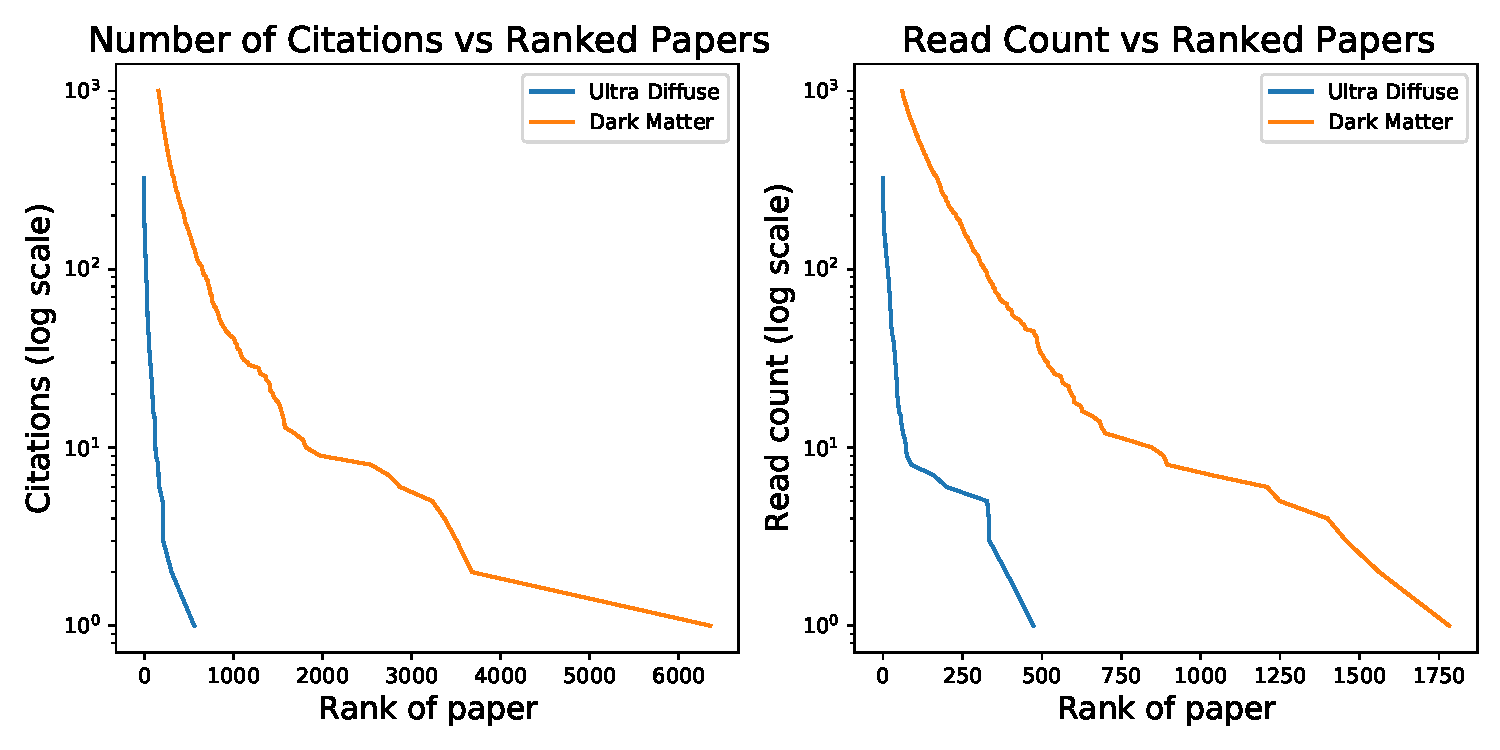
\includegraphics[width =\textwidth]{citeAndRead.pdf}
        %\vspace{-15mm}
        \caption{(a) Left: The top cited papers of all time with the specified keyword appearing in their title, arranged from most cited to least cited.  (b) Right: The top read papers of all time with the specified keyword appearing in their title, arranged from most read to least read. The number of citations is plotted against this in log scale in order to accentuate the characteristics of the curves.}
        \label{fig:y1}
\end{figure}

As shown in Figure \ref{fig:y1}, we can immediately see that dark matter has been a term used amongst scientist for more time than ultra-diffuse galaxies (UDGs), allowing for it to gain appearances in more papers over the year, as well as gaining higher read and citation counts within that pool of papers. Having more time as a popular subject area, will heighten your curve and will cause it to sport a less steep gradient in log space, since less popular papers will still have a chance to gain some level of traction.

\begin{figure}[H]
    \hspace*{-5mm}
        \centering
        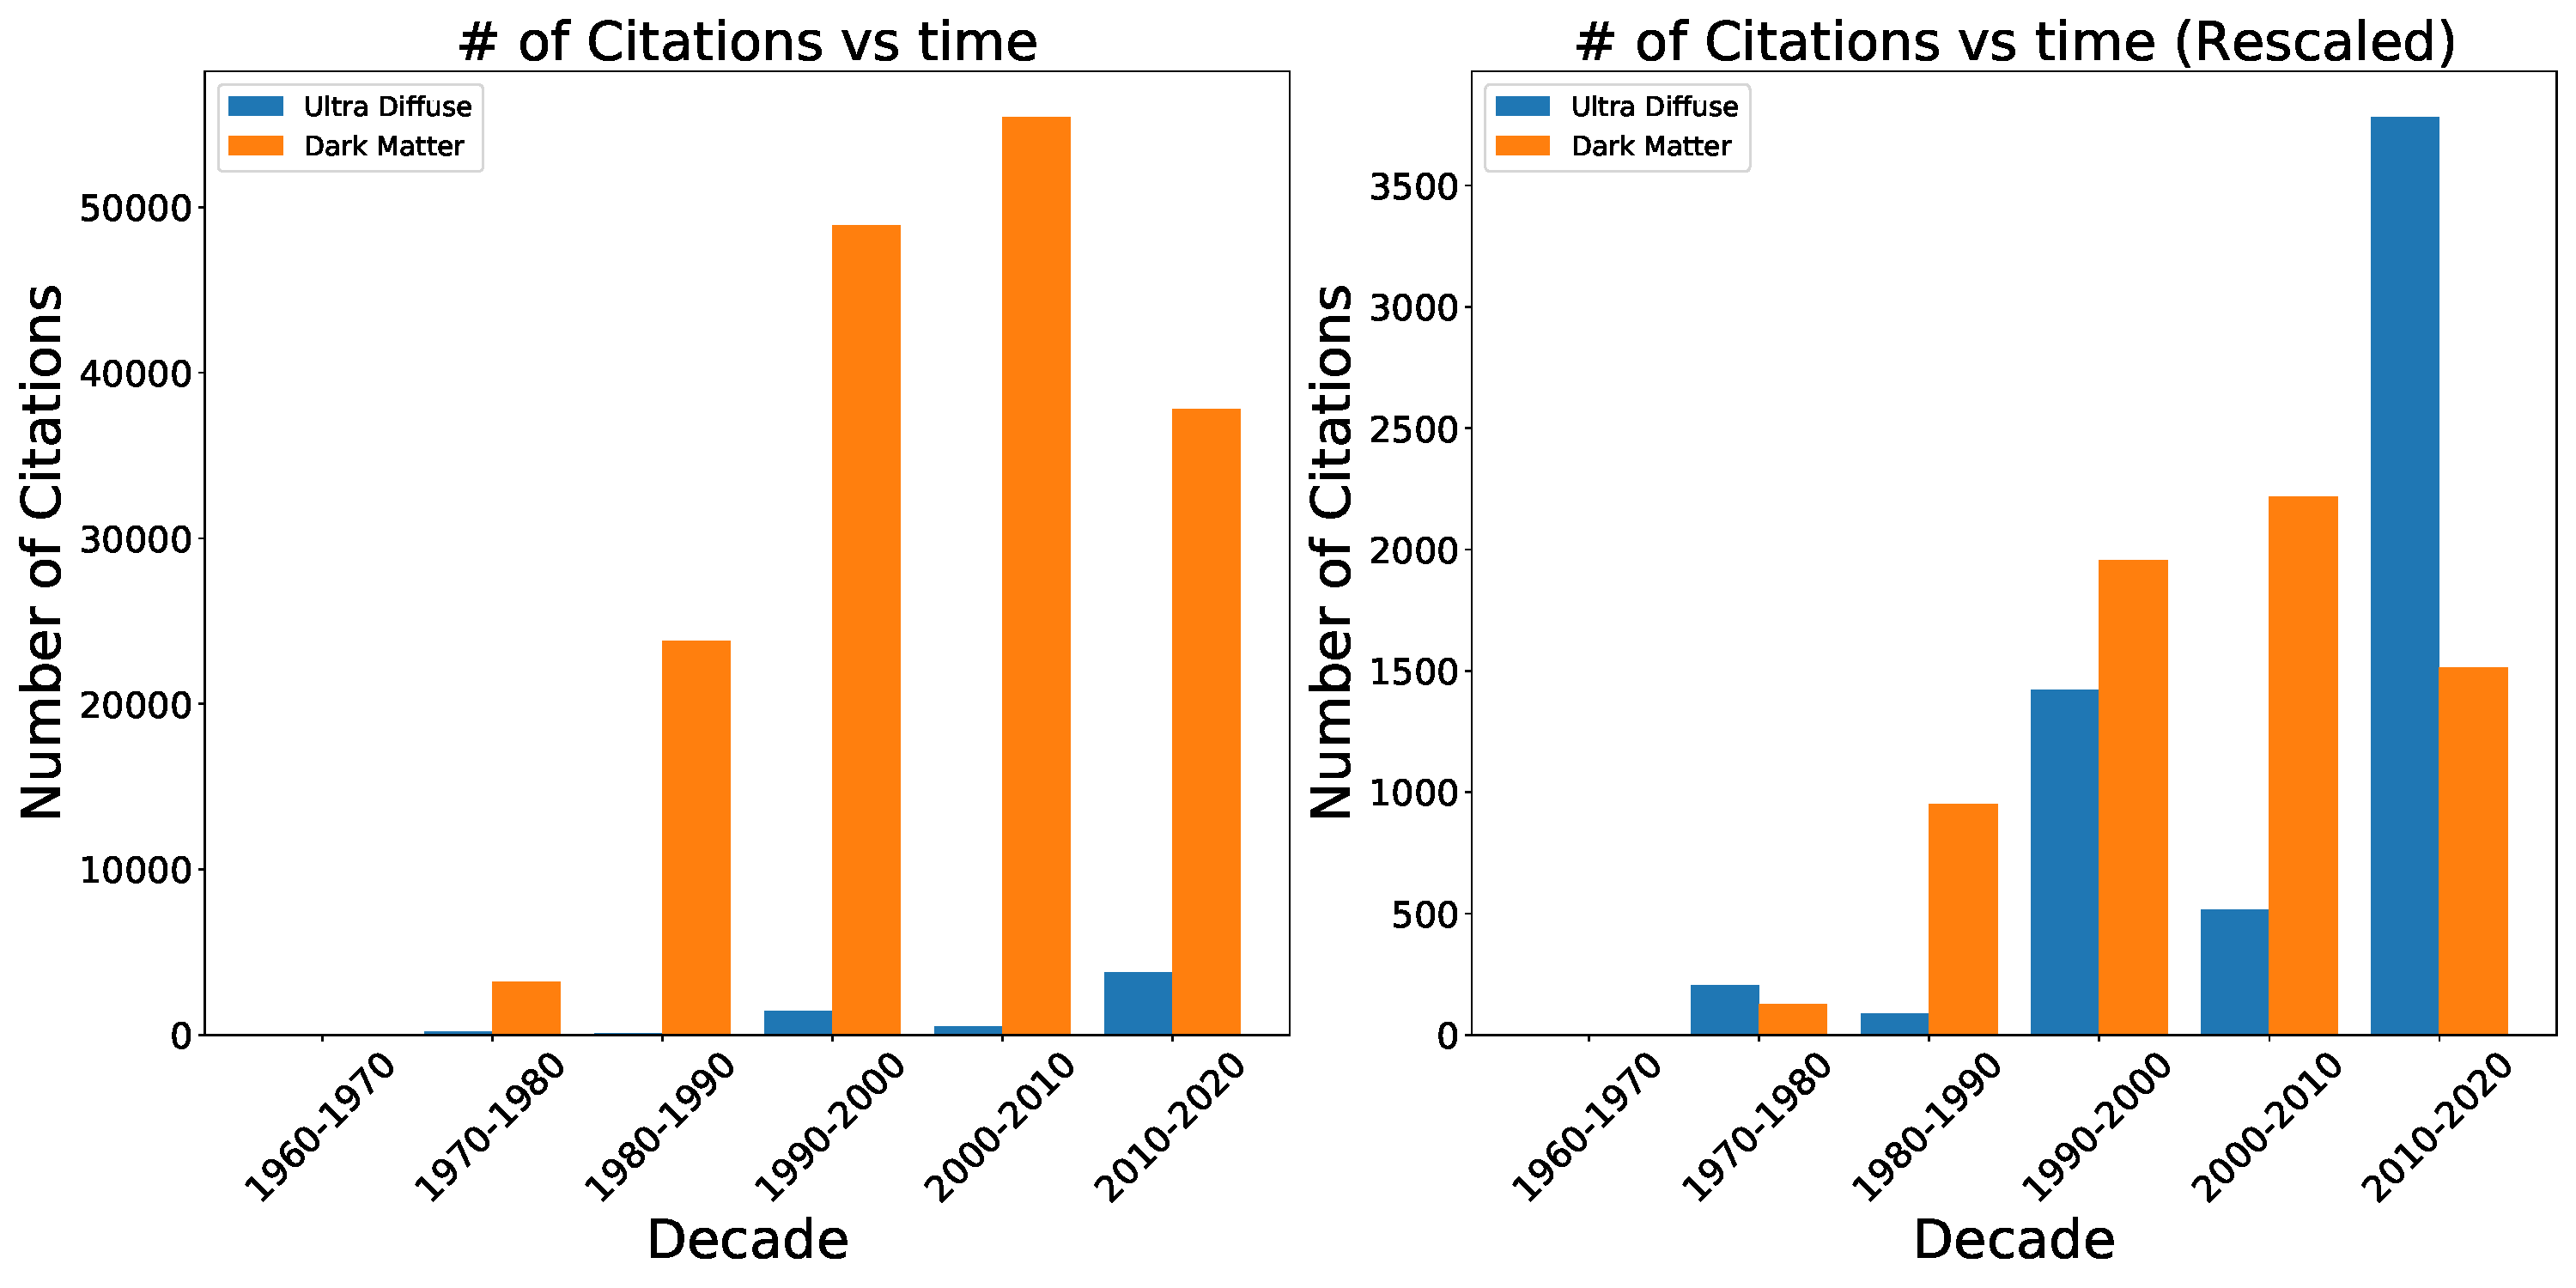
\includegraphics[width =\textwidth]{comparison.pdf}
        %\vspace{-15mm}
        \caption{(a) Left: The number of citations from papers with the keywords 'Dark Matter' and 'Ultra Diffuse Galaxies' in the title, organized in decades from the 1960s to the present day.  (b) Right: Same as the Left but with the Dark Matter data re-scaled by $\dfrac{1}{25}$.}
        \label{fig:y2}
\end{figure}

As seen in Figure \ref{fig:y2}, the trends can be more easily compared when re-scaled to a similar size (plot (b)). From plot (a), we can see that UDGs started to rise in interest a couple decades after dark matter. Since UDGs are difficult to measure and are sometimes comprised of mostly dark matter, it makes sense that the study of dark matter rises in popularity earlier on. From plot (b), We get a sense of how UDGs have completely sky-rocketed in interest over the last decade, while dark matter has decreased slightly. However, this decrease could be an artifact of our query: more recent papers are possibly more likely to contain specific terms related to dark matter in the title, while it being mentioned in the abstract of the body of the paper.



\section{Conclusion}

The \textbf{ads\_query\_pkg} package currently only contains four functions used in order to get a general idea of the trends in interest for any topic in astronomy. However, the functions defined in the package are easily modifiable to suit the specific needs of a user, by simply adding parameters into the ads functions themselves. This creates a large amount of degrees of freedom when it comes to personalizing a function in the \textbf{ads\_query\_pkg} package, and opens up the floor for others to propose different or better ways to analyse and compare interest.

An improvement that should be implemented into these functions appears when checking the papers that are gathered by the \textbf{ads.SearchQuery()} function: a compound keyword is not searched as a single object, but is recognized as two key words being searched independently. This leads to inconveniences related to spelling conventions, e.g. using a hyphen or a space in `Ultra(-/ )Diffuse'.



\end{document}
